\begin{figure*}[tb]
	\begin{minipage}[b]{.2\textwidth}
		\caption{Ouesso-Gruppe: Typvertreter.\\1:~Taf.~54.12; 2:~Taf.~63.7; 3:~Taf.~63.10; 4:~Taf.~63.11; 5:~Taf.~63.9; 6:~Taf.~63.8; 7:~Taf.~65.12; 8:~63.6.}
		\label{fig:OUE_Typvertreter}
	\end{minipage}\hfill
	\begin{minipage}[b]{.8\textwidth}
		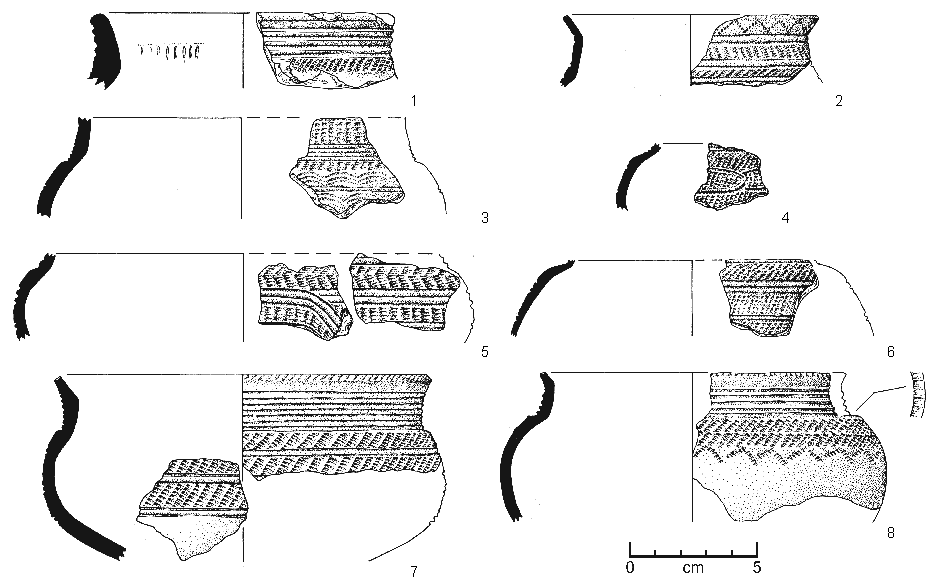
\includegraphics[width=\textwidth]{fig/OUE-Typen.pdf}
		
	\end{minipage}
\end{figure*}

\subsubsection{Ouesso-Gruppe}\label{sec:OUE-Gr}

Die Ouesso-Gruppe umschreibt eine rillen- und kammeindruckverzierte Keramik, die bei Surveys entlang des \mbox{Ngoko} sowie des oberen \mbox{Sangha} gefunden wurde (Abb. \ref{fig:OUE_Verbreitung}). Insgesamt umfasst sie 27 individuell aufgenommene GE und sieben ausgezählte Scherben.\footnote{Die sieben ausgezählten Stücke stammen aus der rezenten Grube PIK~87/2 in Pikunda am \mbox{Sangha} (Kat.-Nr.~9; Fpl.~255). In der Grube fanden sich zudem noch fünf Stücke, die als GE individuell aufgenommen wurden.} Im Inventar des Surveys in Pandama am \mbox{Ngoko} (Fpl.~276) konnten weitere elf GE der Ouesso-Gruppe identifiziert werden.\footnote{Die beiden Fundstellen Pikunda (Fpl.~255) und Pandama (Fpl.~276) lieferten das Gros der Funde der Ouesso-Gruppe. Da aber beide Fundstellen bereits namensgebend für Stile des Arbeitsgebiets sind (Pikunda-Munda; Kap.~\ref{sec:PKM-Gr} und Pandama; Kap.~\ref{sec:PDM-Gr}), wurde die Fundstelle Ouesso am oberen \mbox{Sangha} (Fpl.~265), die zwei GE erbrachte, als eponymer Fundort gewählt.} Alle Funde, mit Ausnahme der genannten Stücke aus Pikunda, stammen aus Oberflächensurveys gegenwärtig bestehender Dörfer.

Die der Ouesso-Gruppe zugewiesenen GE setzen sich vornehmlich aus Wandungsfragmenten zusammen (82~\%), die insbesondere aufgrund ihrer spezifischen Verzierung aus Rillen und Kammeindrücken der Stilgruppe zugewiesen wurden. Randscherben nehmen mit lediglich 18\,\% nur eine untergeordnete Rolle ein. Es sind nur zwei hinreichend vollständige Gefäße (Abb.~\ref{fig:OUE_Typvertreter}.7--8), jedoch keine Bodenstücke bekannt.

\paragraph{Technologische Merkmale}\hspace{-.5em}|\hspace{.5em}%
Die Keramik der Ouesso-Gruppe zeichnet sich mit Blick auf die technologischen Merkmale des Scherben durch deutliche Anteile nichtplastischer Partikel aus. Sichtbare, nichtplastische Partikel sind größtenteils den Korngrößen-Klassen \textit{medium} (44\,\%) und \textit{coarse} (36\,\%) zuzurechnen. Es handelt sich fast ausschließlich um Quarzsande (92\,\%), lediglich in Einzelfällen konnten lateritähnliche oder organische Beimengungen beobachtet werden. Färbungen, die auf die Nutzung rot- oder weißbrennender Tone hindeuten, halten sich mit Anteilen von 22 beziehungsweise 25\,\% in etwa die Waage. Die Hälfte aller Stücke weist graue, schwarze oder beige Färbungen auf, die eine direkte Ansprache der Brennfarbe des genutzten Tones nicht zulassen. Die Keramik der Ouesso-Gruppe ist vornehmlich durch die \textit{Fabrics} 4a (31\,\%), 3c (23\,\%) sowie 4c (23\,\%) repräsentiert.

\paragraph{Formen}\hspace{-.5em}|\hspace{.5em}%
Die Ouesso-Gruppe umfasst nur eine geringe Anzahl GE, zudem konnten lediglich zwei unterschiedliche Gefäßformen festgestellt werden. Bei insgesamt neun GE ließ sich die Gefäßform ansprechen, was lediglich 26\,\% aller Stücke der Stilgruppe entspricht. Bei diesen neun GE handelt es sich um Gefäße mit konvexer Wandung und ausgeprägtem Schulter- und Halsbereich, acht davon sind dem Typ C2 zuzuordnen (Abb.~\ref{fig:OUE_Typvertreter}.3, 5, 7--8) und ein Gefäß mit weniger ausgeprägtem Schulterbereich dem Typ C1. Auffällig ist das regelhafte Vorhandensein eines schmalen Schulterabsatzes (Abb.~\ref{fig:OUE_Typvertreter}.3, 5, 7--8). In einigen Fällen läuft der Absatz auch etwas breiter aus (Abb.~\ref{fig:OUE_Typvertreter}.4, 6). Des Weiteren zeichnen sich die Gefäße durch zylindrische oder kegelförmige Hälse aus. Die Gefäße der Ouesso-Gruppe sind vergleichsweise klein. Der maximale Durchmesser liegt in der Regel zwischen 12--20\,cm. Die Höhe der Mündung konnte nur bei zwei GE hinreichend genau aus dem Verlauf des Profils abgeleitet werden und liegt in beiden Fällen bei 8 beziehungsweise 8,5\,cm. Soweit sich dies aus der kleinen Stückzahl ableiten lässt, sind die Gefäße im Schnitt wohl etwa doppelt so breit wie hoch. Lediglich bei sieben GE konnte die Form des Randes ermittelt werden; sie sind grundsätzlich ausbiegend. Drei GE zeigen einfach ausbiegende (B1; Abb.~\ref{fig:OUE_Typvertreter}.2, 7), drei weitere Stücke leicht konkav ausbiegende Ränder (B2; Abb.~\ref{fig:OUE_Typvertreter}.1) und die letzte GE einen deutlich kurzen, gerade ausbiegenden Rand (B1.1; Abb.~\ref{fig:OUE_Typvertreter}.8). Die Randlippen sind entweder schräg nach außen abgestrichen (M5; 4~GE) oder rund ausgeführt (M1; 2~GE). Fragmente von Böden konnten nicht identifiziert werden.

\begin{figure*}[p]
	\centering
	\includegraphics[width=\textwidth]{fig/OUE_Verbreitung.pdf}
	\caption{Ouesso-Gruppe: Verbreitung \parencite[P1 nach][114 Abb.~42]{Gillet.2013}.}
	\label{fig:OUE_Verbreitung}
\end{figure*}

\paragraph{Verzierungen}\hspace{-.5em}|\hspace{.5em}%
Die Verzierung der GE der Ouesso-Gruppe werden größtenteils von horizontalen Rillen (Tab.~\ref{tab:Verzierungselemente}: 02.1) sowie diagonalem Kammeindruck (Tab.~\ref{tab:Verzierungselemente}: 05.1) bestimmt, die beide jeweils 41\,\% beziehungsweise 40\,\% aller aufgenommen Verzierungselemente der Stilgruppe ausmachen und sich vornehmlich im Schulter- und Bauchbereich der Gefäße finden (Anlage~4\subref{fig:OUE_Verz}). Daneben lassen sich auch horizontale Bänder aus diagonal (Tab.~\ref{tab:Verzierungselemente}: 04.12) sowie vertikal gestellten (Tab.~\ref{tab:Verzierungselemente}: 04.15) Eindrücken beobachten, die etwa 7\,\% aller Verzierungselemente umfassen und sich im Randbereich sowie auf den Gefäßschultern befinden. Grundsätzlich finden sich 35\,\% aller Verzierungselemente auf den Gefäßschultern, gefolgt vom Gefäßbauch (30\,\%) und dem Halsbereich (16\,\%). Die Unterteile der Gefäße sind regelhaft unverziert.


\paragraph{Datierung}\hspace{-.5em}|\hspace{.5em}%
Da keine mit der Keramik assoziierbaren Radiokohlenstoffdatierungen vorliegen und mit Ausnahme der Stücke aus der rezenten Grube PIK~87/2 in Pikunda (Kat.-Nr.~9; Fpl.~255) alle Stücke aus Oberflächenabsammlungen stammen, kann eine chronologische Ansprache der Stilgruppe nur unter Vorbehalt erfolgen. Mit Blick auf stilistische Beziehungen zu anderen Stilgruppen des Arbeitsgebietes ist in erster Linie das regelmäßige Auftreten von schmalen Schulterabsätzen an Keramik der Ouesso-Gruppe zu nennen, was einen Bezug zur Keramik der Stile Ebambe (Kap.~\ref{sec:EBA-Gr}) und Pandama\footnote{Es mag an dieser Stelle darauf hingewiesen werden, dass bei grober Betrachtung des Motivs die diagonalen Kammeindrücke der Ouesso-Keramik (Tab.~\ref{tab:Verzierungselemente}: 05.1) der Verzierung der Keramik der Pandama-Gruppe ähnlich sind; letztere wurde aber mit vegetabilischem \textit{knotted strip}-Roulette erzeugt (Tab.~\ref{tab:Verzierungselemente}: 21.1).} nahelegt (Kap.~\ref{sec:PDM-Gr}). Ein bei Surveys in Pikunda am \mbox{Sangha} gefundenes Gefäß (Taf.~54.7) zeigt weder den ansonsten beobachteten Schulterknick noch die charakteristische Hals- und Randgestaltung. Das Stück deutet aufgrund seines runden Halses und Randes eher auf eine Verwandtschaft zur Konda-Gruppe hin (Kap.~\ref{sec:KON-Gr}). Jedoch zeigt seine Verzierung, die aus mit Rillen gefüllten dreieckigen Flächen und horizontalen Rillen am Rand besteht, eine Ähnlichkeit zur Ouesso-Keramik an. Die Randlippe des genannten Stückes weist, wie auch die Ouesso-Keramik (Abb.~\ref{fig:OUE_Typvertreter}.2,7--8), eine Reihe aus diagonal gesetzten Eindrücken auf. Zusammenfassend kann beim gegenwärtigen Stand eine Datierung im Bereich der Stilgruppen Konda und Pandama, also in die mittlere bis späte Phase der Späten Eisenzeit angenommen werden. Aufgrund dieser Indizien wird für den Ouesso-Stil eine Datierung in das 16.--17.~Jh. n.~Chr. vorgeschlagen.

\paragraph{Verbreitung}\hspace{-.5em}|\hspace{.5em}%
Die Keramik der Ouesso-Gruppe findet sich ausschließlich im Bereich des oberen \mbox{Sangha} sowie dem Gebiet der Einmündung des \mbox{Ngoko} in den \mbox{Sangha} im nordwestlichen Randbereich des Arbeitsgebietes (Abb.~\ref{fig:OUE_Verbreitung}). Der südlichste Fundplatz ist Pikunda am mittleren \mbox{Sangha} (Fpl.~255). Am \mbox{Ngoko} fanden sich GE der Ouesso-Gruppe lediglich in Pandama (Fpl.~276). Der eponyme Fundort Ouesso (Fpl.~265) liegt nur etwas über 25\,km Kilometer südöstlich von Pandama. Nicht eindeutig der Stilgruppe zuweisbare Stücke fanden sich bis nach Bomasa (Fpl.~274), dem stromauf gelegenen Endpunkt der Befahrung des \mbox{Sangha}. Weitere Stücke, die sich potenziell der Ouesso-Gruppe zurechnen lassen, wurden aus dem etwas stromab von Ouesso (Fpl.~265) gelegenen Mboua Mboua berichtet \parencite[114 Abb.~42]{Gillet.2013}.